\chapter{量子光学基础}
\label{chap:03}

\begin{chapteropening}
望远镜收到的是一串点击事件，但这些点击从哪里来？本章的中心问题是：怎样从“光场的状态”走到“探测器记录的事件表”，并判断哪些统计量能在天文观测中保留下来。

最有用的起点不是把光想成一团连续能量，而是把光分解成模式。每个模式有频率、空间形状、偏振和时间范围；光子是模式的激发；探测器记录的是这些模式被吸收后留下的点击。数态、相干态、热态和压缩态分别回答光子数是否固定、相位是否稳定、强度是否涨落、噪声是否能在两个正交分量之间重新分配。单模光子数统计给出成对到达的基线，也决定相关函数在零延迟处的物理含义 \citep{1963PhRv..130.2529G,1963PhRv..131.2766G,1965RvMP...37..231M,1995ocqo.book.....M,1997quop.book.....S,2001qops.book.....S,2013quop.book.....A}。
\end{chapteropening}

\section{望远镜接收到的“一个光子”属于哪个模式}

现在的问题是：当探测器记录一个点击时，这个点击对应的是哪一个自由度？答案不是“一个没有结构的小球”，而是某个光学模式的一次激发。模式可以按频率、时间窗、空间形状、到达方向和偏振来定义。一个窄带、衍射受限、单偏振、持续一个相干时间的场自由度，就是最接近“单模式”的天文例子。

在量子光学里，正频率电场算符可按一组正交模式展开：
\begin{equation}
  \hat E^{(+)}(\bm{r},t)=\sum_k {\cal E}_k u_k(\bm{r})e^{-i\omega_k t}\hat a_k .
  \label{eq:ch03-field-expansion}
\end{equation}
\begin{formulaexplain}
\(\hat E^{(+)}\) 是正频率场算符；\(k\) 标记频率、空间形状和偏振等模式；\({\cal E}_k\) 是模式归一化因子；\(u_k\) 是模式函数；\(\omega_k\) 是角频率；\(\hat a_k\) 是湮灭算符。它把望远镜收到的光写成各个模式的量子激发。
\end{formulaexplain}
这里 \(\hat E^{(+)}\) 是正频率电场算符；\(\bm r\) 是位置，单位厘米；\(t\) 是时间，单位秒；\(\omega_k=2\pi\nu_k\) 是第 \(k\) 个模式的角频率，单位 \(\mathrm{rad\,s^{-1}}\)；\(u_k(\bm r)\) 是空间模式函数；\(\hat a_k\) 是该模式的湮灭算符。标签 \(k\) 不是一个简单序号，而是一整套模式标签：频率、带宽、空间模式、偏振和时间窗。采用不同归一化时，\({\cal E}_k\) 和 \(u_k\) 的量纲可以重新分配，但 \(\hat a_k\) 的量子代数不变。

为什么要引入 \(\hat a_k\)？因为光电探测本质上是在某个模式中减少一个光子。正交模式的产生和湮灭算符满足
\begin{equation}
  [\hat a_i,\hat a_j^\dagger]=\delta_{ij},\qquad
  \hat n_i=\hat a_i^\dagger\hat a_i .
  \label{eq:ch03-commutator}
\end{equation}
\begin{formulaexplain}
\(\hat a_i^\dagger\) 和 \(\hat a_i\) 分别产生、湮灭第 \(i\) 个模式的光子；\(\delta_{ij}\) 表示正交模式；\(\hat n_i\) 是光子数算符。这个对易关系定义了“一个模式里数光子”的量子规则。
\end{formulaexplain}
\(\hat a_i^\dagger\) 往第 \(i\) 个模式里增加一个光子，\(\hat a_i\) 从这个模式里取走一个光子，\(\hat n_i\) 是该模式的光子数算符，本征值 \(N=0,1,2,\ldots\) 没有单位。\(\delta_{ij}\) 表示只有同一模式的产生和湮灭顺序会留下量子修正。望远镜不会直接读出 \(\hat a\) 或 \(\hat E\)，它读出时间戳、像素、能量通道和偏振通道；这些记录是 \(\hat n\) 或多个 \(\hat n\) 的相关函数经过仪器响应后的结果。

天文观测通常不是单模式。若探测窗口长为 \(\Delta t\)，光谱带宽为 \(\Delta\nu\)，望远镜接收的有效光展量为 \(A\Omega\)，偏振通道数为 \(N_{\rm pol}\)，粗略的模式数可写成
\begin{equation}
  M \simeq
  \left(\frac{\Delta t}{\tau_c}\right)
  \left(\frac{A\Omega}{\lambda^2}\right)
  N_{\rm pol},
  \qquad
  \tau_c\simeq\frac{1}{\Delta\nu}\simeq\frac{\lambda^2}{c\,\Delta\lambda}.
  \label{eq:ch03-effective-modes}
\end{equation}
\begin{formulaexplain}
\(M\) 是有效模式数；\(\Delta t/\tau_c\) 数时间模式；\(A\Omega/\lambda^2\) 数空间模式；\(N_{\rm pol}\) 数偏振模式；\(\tau_c\) 是相干时间。它说明实际天文通道常是许多模式的平均。
\end{formulaexplain}
式 \eqref{eq:ch03-effective-modes} 的推法是把可分辨的相空间格子数相乘。一个频带宽度 \(\Delta\nu\) 的波包相干时间约为 \(\tau_c\simeq1/\Delta\nu\)，所以长度为 \(\Delta t\) 的时间窗包含约 \(\Delta t/\tau_c\) 个独立时间模式。空间上，一个衍射受限单模式占据的光展量约为 \(\lambda^2\)，望远镜和后端孔径共接收 \(A\Omega\)，所以空间模式数约为 \(A\Omega/\lambda^2\)。若偏振没有被投影到单一通道，还要乘上偏振模式数 \(N_{\rm pol}\)。最后，\(\nu=c/\lambda\) 给出 \(\Delta\nu\simeq c\,\Delta\lambda/\lambda^2\)，因此 \(\tau_c\simeq\lambda^2/(c\,\Delta\lambda)\)。

\(\Delta t\) 和 \(\tau_c\) 都用秒；\(A\Omega\) 的单位是 \(\mathrm{cm^2\,sr}\)；\(\lambda\) 是波长。式 \eqref{eq:ch03-effective-modes} 只是数量级计数，不是严格的整数公式：真实模式数还会受滤光片形状、点扩散函数、光纤耦合、像素大小和偏振选择影响。衍射受限单空间模式满足 \(A\Omega\sim\lambda^2\)，seeing-limited 光纤或大像素会接收很多空间模式。以 \(\lambda=500\,\mathrm{nm}\)、\(\Delta\lambda=1\,\mathrm{nm}\) 为例，\(\Delta\nu\simeq1.2\times10^{12}\,\mathrm{Hz}\)，所以 \(\tau_c\) 只有约 \(0.8\,\mathrm{ps}\)。若探测器时间响应是 \(100\,\mathrm{ps}\) 到 \(1\,\mathrm{ns}\)，一个时间 bin 已经平均了上百到上千个时间模式 \citep{2000stop.book.....G,1956Natur.177...27B,1957RSPSA.242..300B,1974iiia.book.....H}。

这说明一个重要事实：天文数据中的“一个通道”常常不是一个量子模式，而是许多模式的总和。后面的光子统计、聚束幅度和非经典信号都会被这个模式数稀释。

\section{不同光态怎样改变点击统计}

知道了模式，下一步要问：同一个模式里可以有什么样的光态？最简单的区别不是总光子率，而是计数分布和成对概率。对单模式计数，零延迟成对倾向可用
\[
  b_2\equiv
  \frac{\langle \hat n(\hat n-1)\rangle}{\langle\hat n\rangle^2}.
\]
\(b_2=1\) 是独立 Poisson 到达的基线；\(b_2>1\) 表示聚束；\(b_2<1\) 表示反聚束。数态、相干态和热态即使有相同平均光子数，也会给出不同的 \(P(N)\) 和不同的 \(b_2\)。

数态 \(|n\rangle\) 是光子数算符的本征态：
\begin{equation}
  P_{\rm Fock}(N)=\delta_{Nn},\qquad
  b_2=1-\frac{1}{n}.
  \label{eq:ch03-fock}
\end{equation}
\begin{formulaexplain}
\(P_{\rm Fock}(N)\) 是数态的计数概率；\(\delta_{Nn}\) 表示只可能数到 \(n\) 个光子；\(\hat n\) 是光子数算符；\(b_2\) 衡量同一模式内可组成的光子对数相对独立到达基线的大小。它给出反聚束的理想极限。
\end{formulaexplain}
这里 \(P(N)\) 是数到 \(N\) 个光子的概率。数态的推导最直接：若每次测量都得到 \(N=n\)，则
\[
  \langle \hat n\rangle=n,
  \qquad
  \langle \hat n(\hat n-1)\rangle=n(n-1).
\]
代入成对因子的阶乘矩定义，
\[
  b_{2,{\rm Fock}}
  =
  \frac{n(n-1)}{n^2}
  =
  1-\frac{1}{n}.
\]
单光子态 \(n=1\) 给 \(b_2=0\)，表示不可能在同一模式中同时探测到两个光子，这是反聚束的极限。天体光很少以纯数态到达，因为源区、传播路径和仪器都会混合未观测自由度；但数态告诉我们，点击统计测的是光子数相关，而不是一条连续波形 \citep{1977PhRvL..39..691K,1979OptL....4..205M,1998RvMP...70..101P}。

相干态 \(|\alpha\rangle\) 是稳定相位振荡的理想模型，满足 \(\hat a|\alpha\rangle=\alpha|\alpha\rangle\)。它的平均光子数是 \(\bar n=|\alpha|^2\)，单模计数服从 Poisson 分布：
\begin{equation}
  P_{\rm coh}(N)=e^{-\bar n}\frac{\bar n^N}{N!},
  \qquad
  \operatorname{Var}(N)=\bar n,\qquad
  b_2=1.
  \label{eq:ch03-coherent}
\end{equation}
\begin{formulaexplain}
\(P_{\rm coh}(N)\) 是相干态的 Poisson 计数分布；\(\bar n\) 是平均光子数；\(N!\) 是离散计数归一化；\(\operatorname{Var}(N)=\bar n\) 表示 shot noise；\(b_2=1\) 表示没有额外聚束。
\end{formulaexplain}
\(\alpha\) 是无量纲复振幅；它的模平方给出每个模式的平均光子数，辐角 \(\arg\alpha\) 给出相位。为什么 Poisson 计数会给 \(b_2=1\)？对一个时间窗内的单模计数，成对因子可以写成阶乘矩
\[
  b_2
  =
  \frac{\langle N(N-1)\rangle}{\langle N\rangle^2}.
\]
Poisson 分布的平均数为 \(\bar n\)，其二阶阶乘矩为
\[
  \begin{aligned}
  \langle N(N-1)\rangle
  &=
  \sum_{N=0}^{\infty}N(N-1)e^{-\bar n}\frac{\bar n^N}{N!}  \\
  &=
  e^{-\bar n}\bar n^2
  \sum_{N=2}^{\infty}\frac{\bar n^{N-2}}{(N-2)!}
  =
  \bar n^2 .
  \end{aligned}
\]
代回定义就得到
\[
  b_{2,{\rm coh}}
  =
  \frac{\bar n^2}{\bar n^2}=1 .
\]
这一步的物理意思是：扣除“同一个光子不能被数两次”的自配对以后，Poisson 光的光子对数正好等于独立到达给出的随机基线。看到一个光子，并不会提高同一模式中马上再看到一个光子的条件概率。稳定实验室激光在许多测量中接近相干态；天体窄线或高亮温源却不自动是相干态，因为独立发射区、速度场和散射路径会把相位平均掉。

热态是天体连续谱最常用的起点。单模热态的密度矩阵为
\begin{equation}
  \rho_{\rm th}=\sum_{N=0}^{\infty}
  \frac{\bar n^N}{(1+\bar n)^{N+1}}|N\rangle\langle N|,
  \qquad
  \operatorname{Var}(N)=\bar n(1+\bar n),\qquad
  b_2=2.
  \label{eq:ch03-thermal-density}
\end{equation}
\begin{formulaexplain}
\(\rho_{\rm th}\) 是热态密度矩阵；\(|N\rangle\) 是 \(N\) 光子数态；\(\bar n\) 是单模平均占有数；\(\operatorname{Var}(N)\) 是计数方差。它说明热光是光子数混合态，并自然产生 \(b_2=2\) 的聚束。
\end{formulaexplain}
这里 \(\bar n\) 是单模式平均占有数，不是望远镜每秒收到的总光子率。热态没有固定相位，是光子数基底上的混合态。式 \eqref{eq:ch03-thermal-density} 中的计数分布是几何分布。它的平均和方差为
\[
  \langle N\rangle=\bar n,
  \qquad
  \operatorname{Var}(N)=\langle N^2\rangle-\langle N\rangle^2
  =\bar n(1+\bar n).
\]
二阶相关需要的是 \(\langle N(N-1)\rangle\)，而不是普通的 \(\langle N^2\rangle\)。二者关系为
\[
  \langle N(N-1)\rangle
  =
  \langle N^2\rangle-\langle N\rangle
  =
  \operatorname{Var}(N)+\langle N\rangle^2-\langle N\rangle .
\]
把热态的平均和方差代入，
\[
  \langle N(N-1)\rangle
  =
  \bar n(1+\bar n)+\bar n^2-\bar n
  =
  2\bar n^2 ,
\]
所以
\[
  b_{2,{\rm th}}
  =
  \frac{2\bar n^2}{\bar n^2}=2 .
\]
这多出来的一倍不是探测器效应，而是热光强度涨落本身带来的成对概率增强：某一小段时间里强度偏高时，多个光子会一起更容易到来；强度偏低时，它们又一起变少。多模热光会把这种过量方差平均掉，使实际观测到的聚束对比度小于单模理想值 \citep{1965RvMP...37..231M,1995ocqo.book.....M,2000stop.book.....G,2017MNRAS.472.4126G,2024arXiv240418606N}。

\begin{figure}[tbp]
\centering
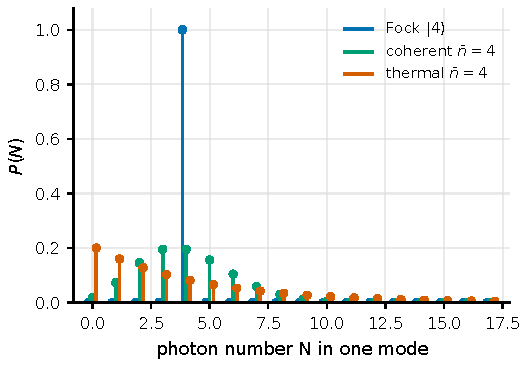
\includegraphics[width=0.82\linewidth]{figures/generated/chapter_03/ch03_state_count_distributions.pdf}
\caption{同一单模平均光子数附近，数态、相干态和热态给出完全不同的计数分布。数态的光子数固定，相干态的宽度为 \(\sqrt{\bar n}\)，热态有更长的高光子数尾部，所以会产生 \(b_2>1\) 的聚束信号。}
\label{fig:ch03-count-distributions}
\end{figure}

图 \ref{fig:ch03-count-distributions} 的物理意思很简单：平均光子数不是全部。数态没有光子数涨落；相干态有 Poisson 涨落；热态有额外强度涨落。天文强度干涉利用的正是最后这种热光涨落。

压缩态说明另一件事：量子噪声可以在两个正交场分量之间重新分配。定义
\begin{equation}
  \hat X_\theta=\frac{1}{2}\left(\hat a e^{-i\theta}+\hat a^\dagger e^{i\theta}\right),
  \qquad
  \Delta X_{\rm sq}^2=\frac{1}{4}e^{-2r},\qquad
  \Delta X_{\rm anti}^2=\frac{1}{4}e^{2r}.
  \label{eq:ch03-squeezing}
\end{equation}
\begin{formulaexplain}
\(\hat X_\theta\) 是相位角 \(\theta\) 上的场正交分量；\(r\) 是压缩参数；\(\Delta X_{\rm sq}^2\) 和 \(\Delta X_{\rm anti}^2\) 是被压低和被抬高的方差。它说明压缩态把噪声在两个共轭方向间重新分配。
\end{formulaexplain}
\(\hat X_\theta\) 是无量纲正交分量，真空噪声方差为 \(1/4\)，\(r\) 是压缩参数。这个方差形式来自单模压缩变换：沿一个正交方向的振幅尺度乘上 \(e^{-r}\)，方差就乘上 \(e^{-2r}\)；共轭方向的尺度乘上 \(e^{r}\)，方差就乘上 \(e^{2r}\)。两者乘积仍为
\[
  \Delta X_{\rm sq}^2\,\Delta X_{\rm anti}^2
  =
  \frac{1}{16},
\]
说明压缩态没有消灭量子噪声，而是把噪声从一个正交方向转移到另一个方向。实验论文常用 dB 表示噪声方差相对真空的比例，例如 \(10\log_{10}(e^{-2r})=-10\,\mathrm{dB}\) 表示方差降为真空的十分之一。现代压缩光实验已经在 \(1064\,\mathrm{nm}\) 附近测得 10 到 15 dB 量级的噪声降低，并用于引力波探测器和量子效率标定；但普通恒星连续谱并不默认具有压缩 \citep{1983Natur.306..141W,1987JMOp...34..709L,2016PhRvL.117k0801V}。

\begin{figure}[tbp]
\centering
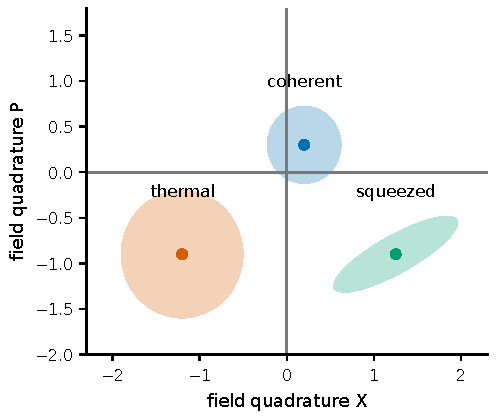
\includegraphics[width=0.72\linewidth]{figures/generated/chapter_03/ch03_phase_space_states.pdf}
\caption{相空间中三类常见单模光态的宽度。相干态的噪声接近真空圆斑，热态因随机强度和相位而变宽，压缩态把一个正交分量的涨落压低，同时把共轭分量的涨落抬高。}
\label{fig:ch03-phase-space}
\end{figure}

相空间图把一个模式写成两个正交分量 \(X\) 和 \(P\) 的概率图像。相干态像真空噪声大小的圆斑，只是圆心移动；热态仍近似圆形，但半径由 \(\bar n\) 放大；压缩态在一个方向变窄、另一个方向变宽。这个图像能帮助我们记住：不同光态的区别首先表现为涨落和相关，而不只是平均强度。

\section{为什么天体光通常要用密度矩阵和弱热光近似}

如果一个系统的所有自由度都被完整保留，可以用纯态描述。但天文观测几乎总是丢掉一些自由度：带外频率没记录，偏振可能没分辨，seeing 把空间模式混在一起，长时间 bin 把许多相干时间内的涨落加在一起。因此真正用于数据分析的状态通常是混合态。

相空间语言可以把这种混合写成不同表示。Glauber--Sudarshan \(P\) 表示把密度矩阵写成相干态混合，\(Q\) 函数对应异频探测时被真空噪声平滑后的分布：
\begin{equation}
  \rho=\int P(\alpha)|\alpha\rangle\langle\alpha|\,\mathrm{d}^2\alpha,
  \qquad
  Q(\alpha)=\frac{1}{\pi}\langle\alpha|\rho|\alpha\rangle .
  \label{eq:ch03-phase-space}
\end{equation}
\begin{formulaexplain}
\(\rho\) 是密度矩阵；\(P(\alpha)\) 是相干态混合权重；\(|\alpha\rangle\) 是相干态；\(Q(\alpha)\) 是由 \(\rho\) 投影得到的相空间分布。这个式子把“经典随机场”和“量子态”之间的边界写清楚。
\end{formulaexplain}
若 \(P(\alpha)\) 是正常的非负概率密度，许多强度和相干函数可以用经典随机场得到同样结果；热光和相干光在这个意义上常常是“经典”的。若 \(P\) 比 delta 函数还奇异，或 Wigner 函数出现负值，半经典图像就会失效。天体强度干涉的大部分基础公式处在半经典和量子理论等价的区域，但探测、损耗和弱光极限仍然更适合用密度矩阵记账 \citep{1963PhRvL..10..277S,1972PhRvA...6.2211A,2001qops.book.....S,1996PhRvL..76.4344B,1999PhRvA..60..674B}。

把未记录自由度丢掉的数学操作是 partial trace：
\begin{equation}
  \rho_{\rm obs}=\operatorname{Tr}_{\rm unobs}\rho_{\rm full}.
  \label{eq:ch03-partial-trace}
\end{equation}
\begin{formulaexplain}
\(\rho_{\rm full}\) 是包含所有自由度的完整状态；\(\operatorname{Tr}_{\rm unobs}\) 表示对未观测标签求迹；\(\rho_{\rm obs}\) 是数据实际保留的状态。它把“没有记录的信息要平均掉”写成密度矩阵操作。
\end{formulaexplain}
\(\rho_{\rm full}\) 可以包含源区位置、频率、传播路径、偏振、探测器内部自由度和环境；\(\rho_{\rm obs}\) 只保留数据中还可区分的自由度。这个公式说的不是抽象哲学，而是数据处理事实：没有记录的标签不能在似然函数里被当成可区分信息。宇宙学涨落退相干、引力透镜路径相干性限制和恒星强度干涉的视直径退相干，数学上都在处理“保留哪些自由度、平均掉哪些自由度”的问题 \citep{1998RvMP...70..101P,2020MNRAS.491.5789L,1996CQGra..13..377P}。

天体弱光极限还需要另一个数量级。热辐射的单模占有数由亮温 \(T_b\) 给出：
\begin{equation}
  \bar n_\nu=\frac{1}{\exp(h\nu/k_{\rm B}T_b)-1}.
  \label{eq:ch03-occupation}
\end{equation}
\begin{formulaexplain}
\(\bar n_\nu\) 是频率 \(\nu\) 的单模平均占有数；\(h\nu\) 是光子能量；\(k_{\rm B}T_b\) 是亮温对应的热能。它说明总光子率很高并不等于每个光学模式里有很多光子。
\end{formulaexplain}
\(h\nu\) 和 \(k_{\rm B}T_b\) 都是能量，单位 erg；\(\bar n_\nu\) 无量纲。式 \eqref{eq:ch03-occupation} 是单个玻色模式的 Bose--Einstein 占有数：光子数为 \(N\) 的能量为 \(Nh\nu\)，热权重按 \(\exp(-Nh\nu/k_{\rm B}T_b)\) 递减，归一化后得到几何分布；对这个分布求平均就得到 \(\bar n_\nu=[\exp(h\nu/k_{\rm B}T_b)-1]^{-1}\)。对 \(T_b=5800\,\mathrm{K}\) 的恒星表面，\(\lambda=500\,\mathrm{nm}\) 时 \(h\nu/k_{\rm B}T_b\simeq5\)，\(\bar n_\nu\simeq7\times10^{-3}\)；到 \(1\,\mu\mathrm{m}\) 时 \(\bar n_\nu\simeq0.09\)；到 \(10\,\mu\mathrm{m}\) 时可超过 1。射电和毫米波因为 \(h\nu\ll k_{\rm B}T_b\)，常进入高占有数、近经典波动的 Rayleigh--Jeans 区域。这个数量级解释了为什么光学天文可以有很高总光子率，却仍常处在每模式弱光极限。

\begin{figure}[tbp]
\centering
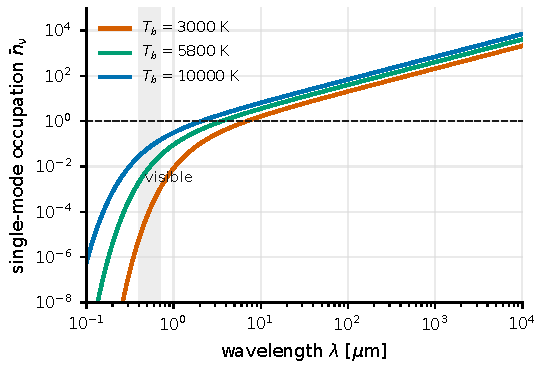
\includegraphics[width=0.82\linewidth]{figures/generated/chapter_03/ch03_blackbody_mode_occupation.pdf}
\caption{不同亮温黑体的单模占有数随波长变化。可见光灰带内，即使 \(T_b\) 为太阳量级，\(\bar n_\nu\) 也远小于 1；红外、毫米波或高亮温 maser 区域则可以进入 \(\bar n_\nu\gtrsim1\) 的强占有数极限。}
\label{fig:ch03-mode-occupation}
\end{figure}

在光学弱热光中，每个相干时间窗内常常没有光子，少数窗有一个光子。这个情况可写成
\begin{equation}
  \rho\simeq (1-\epsilon)\rho_0+\epsilon\rho_1+O(\epsilon^2),
  \qquad
  \epsilon\equiv\langle N\rangle_{\rm mode}\ll1.
  \label{eq:ch03-weak-thermal}
\end{equation}
\begin{formulaexplain}
\(\rho_0\) 是真空部分；\(\rho_1\) 是一光子部分；\(\epsilon\) 是单模式平均计数；\(O(\epsilon^2)\) 是双光子及更高项。弱热光极限下，大部分时间窗为空，少数点击携带空间和时间信息。
\end{formulaexplain}
\(\rho_0\) 是真空项，\(\rho_1\) 是一光子项，\(\epsilon\) 是该模式在该时间窗内的平均光子数。这个展开来自热态计数分布在 \(\bar n\ll1\) 时的最低阶：
\[
  P(0)=\frac{1}{1+\bar n}\simeq1-\bar n,
  \qquad
  P(1)=\frac{\bar n}{(1+\bar n)^2}\simeq\bar n,
  \qquad
  P(N\ge2)=O(\bar n^2).
\]
因此可以把 \(\epsilon\) 识别为单模式平均光子数。Tsang、Nair 和 Lu 的弱热光超分辨理论正是从这个展开出发：大多数相干时间窗没有点击，真正携带空间信息的是被探测到的一光子模式 \citep{1969JSP.....1..231H,2015Optic...2..646T,2016PhRvX...6c1033T}。这和天文事件表很吻合：零光子时间窗通常不会存入文件，留下来的是带时间戳的点击。

\section{光态怎样进入探测语言}

光场状态只有通过探测器才变成数据。理想光电探测器通过吸收光子产生点击，所以点击概率由场中的湮灭算符和产生算符按吸收事件的顺序组合而成。这个顺序通常叫正规序，它自动去掉“同一个光子和自己配对”的假项，因此单模二阶计数会出现 \(\langle \hat n(\hat n-1)\rangle\)，而不是普通的 \(\langle \hat n^2\rangle\)。

正规序给出的单模关系与 \(b_2\) 的定义一致。若只看一个模式，正频率场与湮灭算符成正比，\(\hat E^{(+)}\propto\hat a\)。一次点击对应一个吸收事件，两个点击对应两个吸收事件；于是平均计数与 \(\langle\hat a^\dagger\hat a\rangle=\langle\hat n\rangle\) 成正比，成对计数与 \(\langle\hat a^\dagger\hat a^\dagger\hat a\hat a\rangle=\langle\hat n(\hat n-1)\rangle\) 成正比。多通道、有限时间响应、背景和死时间会改变观测到的相关峰形和归一化，但不会改变“两个点击对应两个吸收事件”这个基本计数规则 \citep{1963PhRv..130.2529G,1965RvMP...37..231M,1995ocqo.book.....M,2017MNRAS.472.4126G}。

\section{非经典边界和天体 maser}

天体光能否表现出真正非经典统计？对单模式计数，最简单的边界是 \(b_2<1\)：同时探测两个光子的概率低于 Poisson 光，不能用正的经典强度涨落解释。实验室里的共振荧光和单光子源可以清楚地产生反聚束；天体观测却要面对多源混合、传播模式混合、背景和暗计数。即使某个微观过程发出非经典光，只要观测时无法隔离单个发射体和单个模式，最后的观测成对统计往往会被拉回 Poisson 基线 \citep{1977PhRvL..39..691K,1979OptL....4..205M,1995ocqo.book.....M}。

\begin{figure}[tbp]
\centering
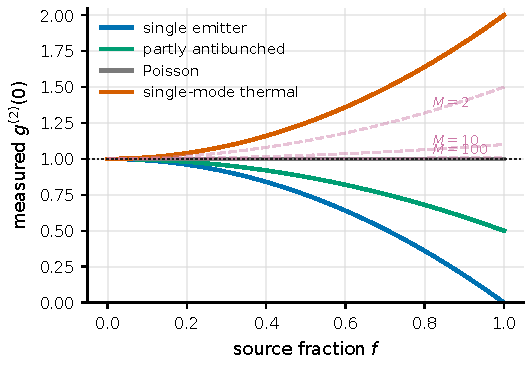
\includegraphics[width=0.74\linewidth]{figures/generated/chapter_03/ch03_nonclassical_mixing_boundary.pdf}
\caption{背景和多源混合会把观测到的成对统计拉向 Poisson 基线。蓝线表示理想单发射体反聚束，橙线表示单模热光聚束；源光子比例 \(f\) 下降时，偏离 1 的幅度按 \(f^2\) 变小。虚线显示多模热光 \(M>1\) 的聚束峰也会随模式数增大而变浅。}
\label{fig:ch03-nonclassical-mixing}
\end{figure}

受激辐射、maser 和 astrophysical laser 是容易被误说的边界情况。受激辐射可以给很高亮温和很窄线宽，射电 maser 的单模占有数可以非常大；但高亮温不等于相干态，窄线也不自动给 Poisson 成对统计。未饱和 maser、饱和 maser、多个斑点叠加、速度梯度和泵浦噪声会产生不同时间统计。若要用 photon correlation spectroscopy 区分自然 laser 成分，必须同时给出线宽、空间相干、偏振、背景连续谱和仪器时间响应，不能只凭“非 Poisson”判断新物理 \citep{1972ApJ...174..517G,2005NewA...10..361J,2008AIPC..984..216D,2017MNRAS.472.4126G}。

\begin{longtable}{p{0.16\linewidth}p{0.22\linewidth}p{0.20\linewidth}p{0.25\linewidth}}
\toprule
光态 & 单模计数 & \(b_2\) & 天文语境 \\
\midrule
数态 \(|n\rangle\) & 固定 \(N=n\) & \(1-1/n\) & 单发射体或量子源的理想模型，天体上极难隔离。 \\
相干态 & Poisson & 1 & 稳定激光的近似；天体窄线不必然是相干态。 \\
热态 & Bose--Einstein & 2 & 恒星连续谱和许多非相干源的基本模型；多模和仪器响应会降低观测对比度。 \\
压缩态 & 取决于测量正交量 & 可大于、小于或接近 1 & 仪器量子噪声工程重要，普通天体光不默认具有压缩。 \\
\bottomrule
\end{longtable}
